%=========================================================================
%=========================================================================
\chapter{DVD Contents}

Following files can be found on the attached DVD:

{\renewcommand{\arraystretch}{1.2}
\begin{table}[htbp]
	\centering
	\begin{tabularx}{1.0\textwidth}{lX}
		\textbf{/text} & Source files of this work (.tex), the figures and the final document (.pdf). \\
		\textbf{/poster} & The poster of this work presented at conference Excel@FIT 2016 (A1 format, .pdf). \\
		\textbf{/video} & The video  overviewing this work presented at conference Excel@FIT 2016 (.mp4, h264). \\
		\textbf{/paper} & The paper published at conference Excel@FIT 2016 (.pdf). \\
		\textbf{/ols/src} & Source code of the OLS divided into separate ROS packages (.cpp, .h, other auxiliary formats). \\
		\textbf{/ols/data} & Part of the meadow dataset included (.bag). \\
		\textbf{/ols/doc} & The generated documentation of the source code (.html). \\
		\textbf{/misc/photos} & Various photographs of the OLS taken during development, rectification and testing (.jpg). \\
		\textbf{/misc/videos} & Various videos documenting the development and testing of the OLS (.mp4, h264). \\
		\textbf{/README.txt} & Text file including the description of the DVD contents, system requirements, building and running instructions and the usage manual. \\
	\end{tabularx}
	\label{tab:dvd_contents}
\end{table}%
}

%=========================================================================
%=========================================================================
\chapter{Usage of the OLS}
- mozna pridat jeste Building, Running, nebo to dat az do readme.txt

%=========================================================================
%=========================================================================
\chapter{Paper - Excel@FIT 2016}

\includepdf[pages={1,2,3,4,5,6,7,8}, offset=50 -45]{appendix/2016-ExcelFIT-paper.pdf}

%=========================================================================
%=========================================================================
\chapter{Poster - Excel@FIT 2016}

\begin{figure}[htp] 
	\centering {
		\vspace*{-1.5cm}
		\hspace*{-2.2cm}
		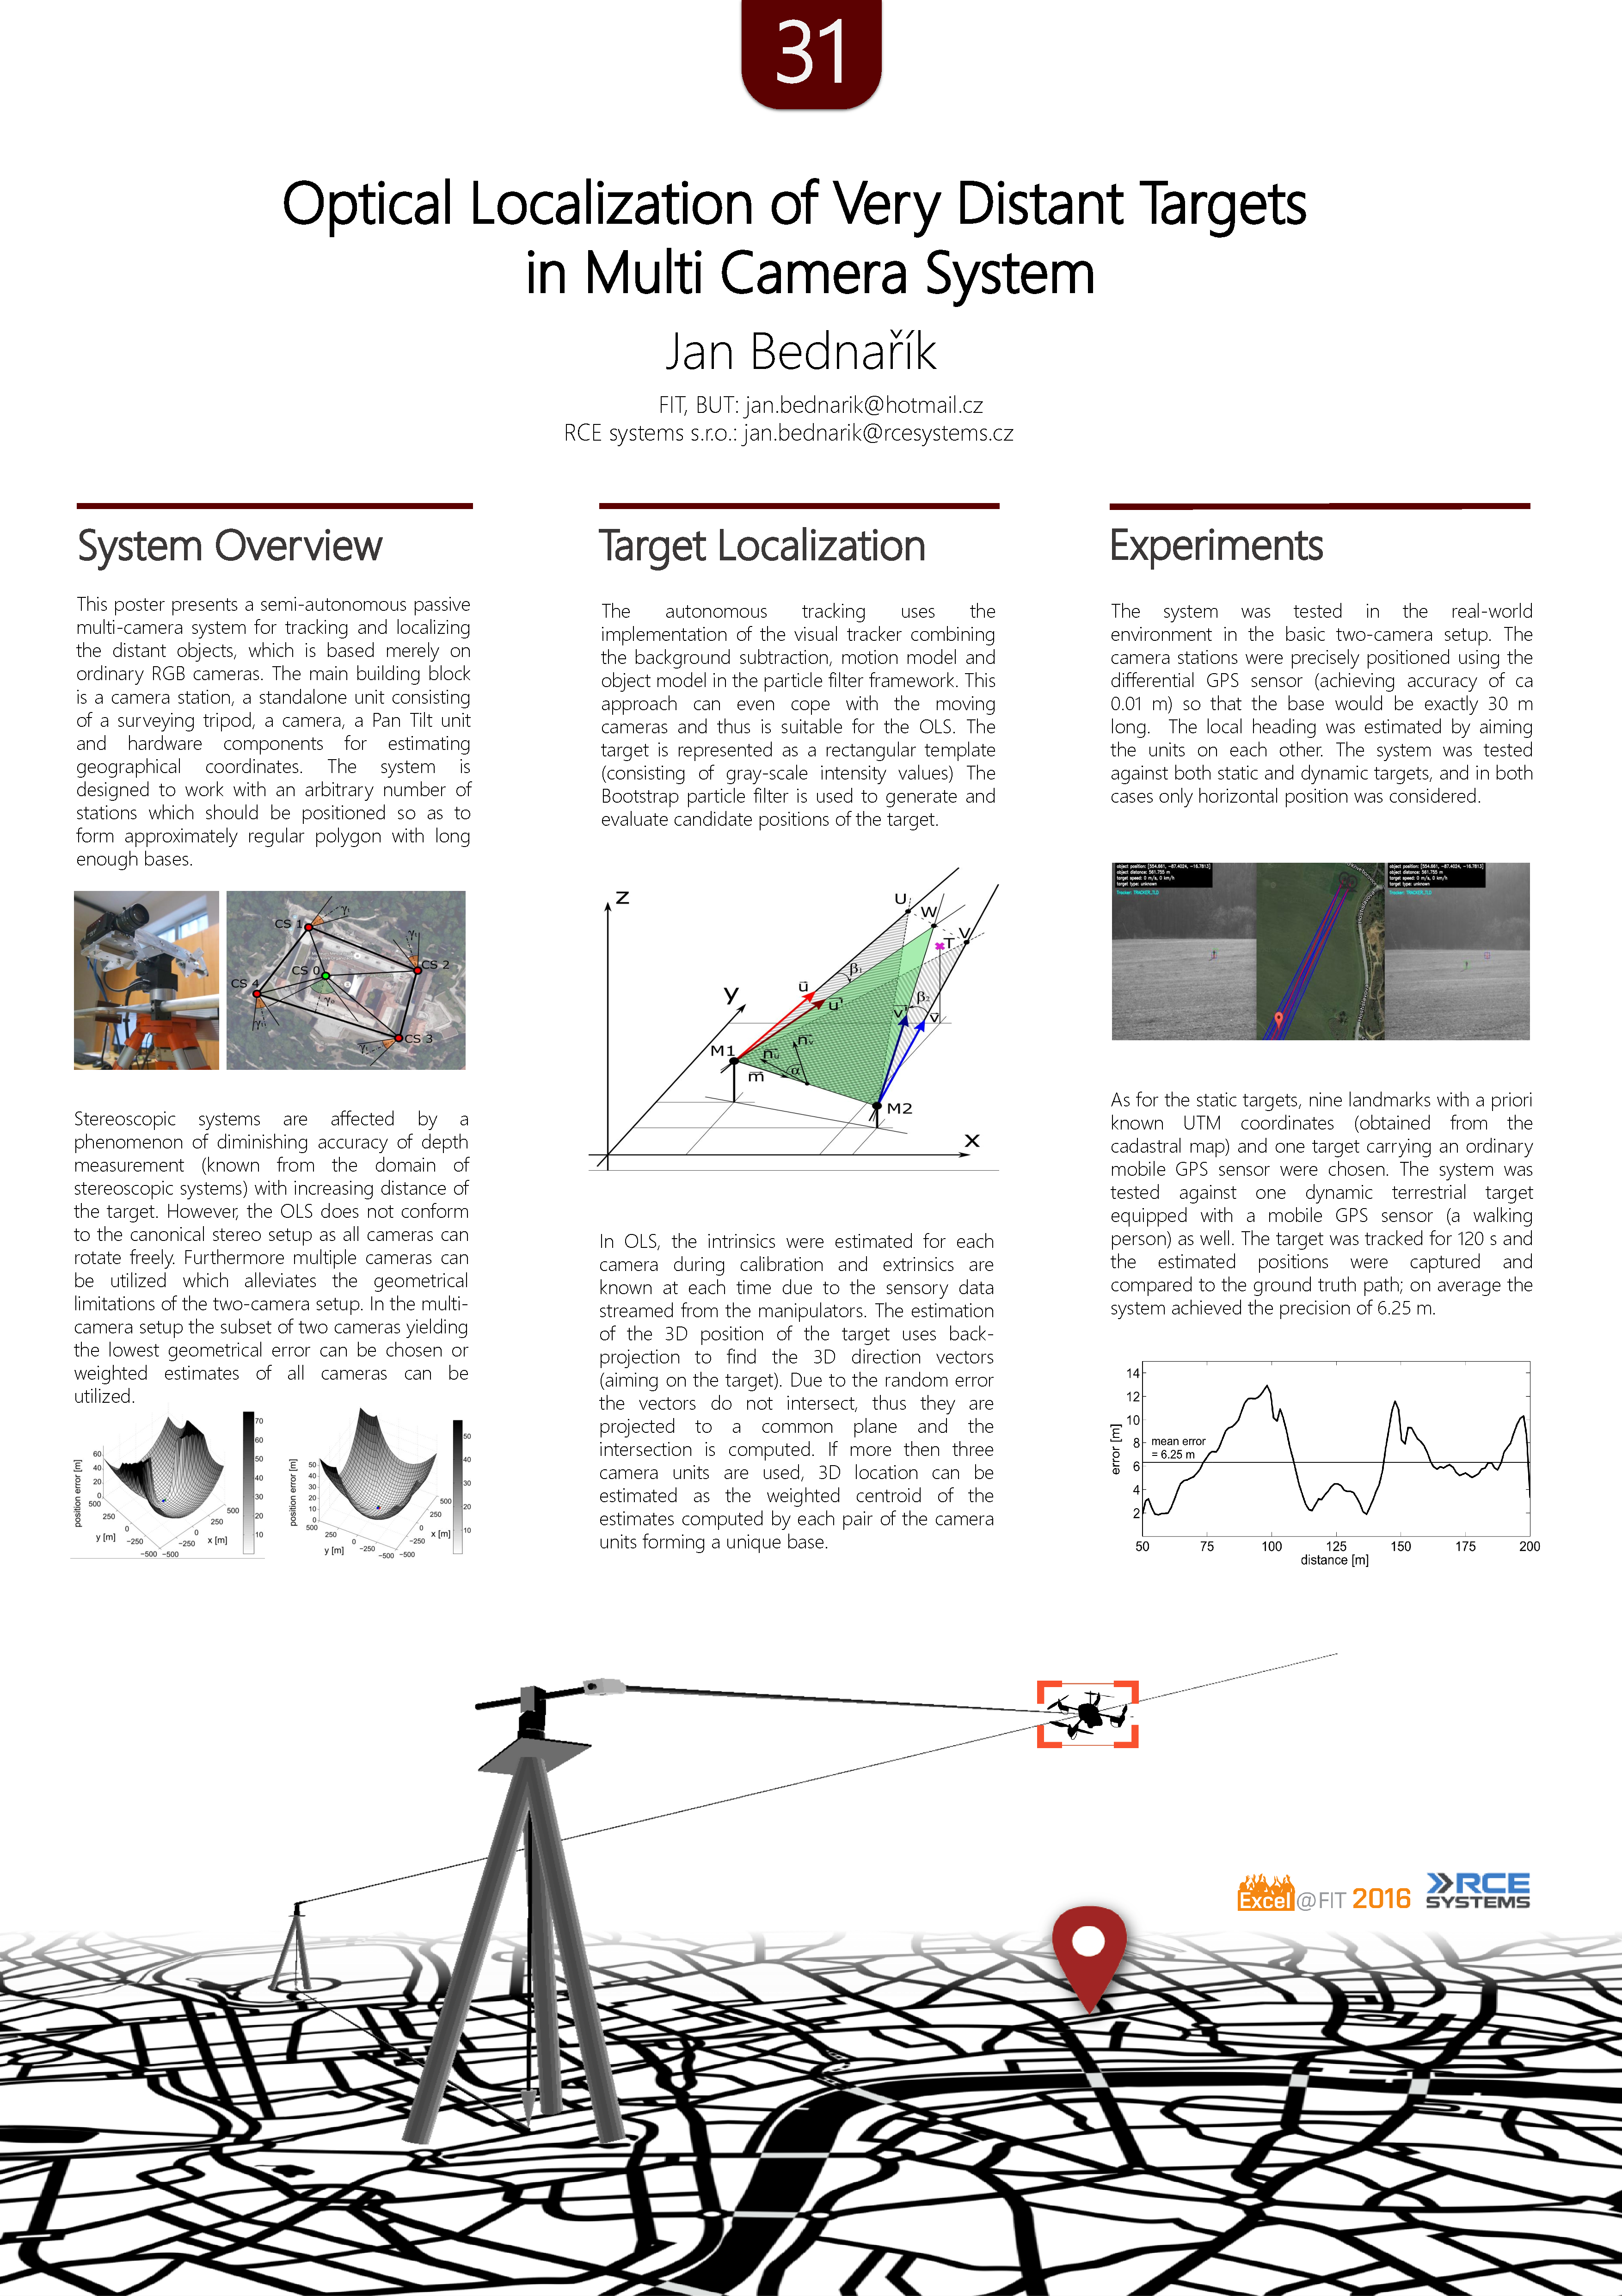
\includegraphics[scale=0.32]{appendix/2016-ExcelFIT-poster.pdf}
	}
\end{figure}